\documentclass[11pt,a4paper]{article}
\usepackage[T1]{fontenc}
\usepackage[utf8]{inputenc}
\usepackage[spanish,es-noshorthands]{babel}
\usepackage{amsmath,amssymb,bm}
\usepackage{graphicx,booktabs,hyperref,geometry,enumitem}
\usepackage{siunitx}
\geometry{margin=2.4cm}
\graphicspath{{../../results/tmm/}}
\hypersetup{colorlinks=true,linkcolor=black,citecolor=blue,urlcolor=blue}
\setlist[itemize]{topsep=0.3em,itemsep=0.15em}
\setlist[enumerate]{topsep=0.3em,itemsep=0.15em}

\title{Guía conceptual de la replicación:\\
plasmon-polaritones en superredes Fibonacci de metamaterial}
\author{Emanuel Orozco Gallego}
\date{31 de agosto de 2026}

\begin{document}
\maketitle

\begin{abstract}
Este documento explica, desde cero y sin omitir pasos, toda la física que hay
detrás de la reimplementación de E.~Reyes-Gómez \textit{et al.},
Phys.\ Rev.\ B \textbf{81}, 153101 (2010).
No es un resumen del código: es el mapa conceptual que hace falta para entender
\emph{qué} se está calculando, \emph{por qué} esas magnitudes existen y
\emph{qué} significan las seis figuras del original.
La solución numérica y el recorrido del código viven en el documento hermano
\textit{Solución numérica e implementación}.
\end{abstract}

\tableofcontents
\newpage

\section{Cómo leer este texto}

Si es la primera vez que estudia fotónica, metamateriales o superredes
cuasiperiódicas, el orden de las secciones está pensado para no dar nada por
sabido. Cada idea nueva se apoya solo en las anteriores.

Convenciones que se usan en todo el proyecto:

\begin{itemize}
\item \(\omega\): frecuencia \emph{angular}, en radianes por segundo.
\item \(\nu=\omega/(2\pi)\): frecuencia cíclica. Es la que aparece en los ejes
de las figuras, en gigahercios (GHz).
\item Nunca se mezcla \(f\) con \(\omega\). Si el paper escribe
\(\omega_e/2\pi=3\,\mathrm{GHz}\), eso significa
\(\nu_e=3\,\mathrm{GHz}\) y \(\omega_e=2\pi\times 3\times 10^9\,\mathrm{rad/s}\).
\item Las afirmaciones que están \emph{escritas} en el PRB de 2010 se tratan
como fuente primaria. Donde el paper omite un factor o una matriz, se dice
explícitamente y se indica de dónde se restauró (casi siempre el artículo
hermano del mismo grupo, EPL \textbf{88}, 24002, 2009).
\end{itemize}

El sistema físico, en una frase: una superred unidimensional periódica cuya
\emph{celda} no es el dímero \(AB\), sino una palabra de Fibonacci hecha de
aire y de un metamaterial Drude; a incidencia oblicua TE, la luz se acopla a
oscilaciones magnéticas de ese metamaterial y aparecen modos llamados
plasmon-polaritones.

\section{Qué replica el proyecto}

El artículo original es un Brief Report de cuatro páginas.
Estudia cómo se organizan esos modos cuando la celda elemental sigue una
secuencia de Fibonacci, en lugar de un apilamiento periódico simple \(ABAB\ldots\)

Lo que el proyecto reproduce no es una paráfrasis del texto, sino el
\emph{cálculo}: las mismas ecuaciones, los mismos parámetros publicados y las
mismas seis figuras, obtenidas con el método de matriz de transferencia (TMM).
No se usa FDTD ni elementos finitos.

Pregunta física del paper, traducida:

\begin{quote}
Si apilo aire y un metamaterial de índice negativo según Fibonacci, y ilumino
en oblicuo con polarización TE, ¿cuántos modos acoplados luz--plasmón aparecen
y cómo se fragmentan al subir el orden de Fibonacci?
\end{quote}

La respuesta del original, que el código verifica número a número, es:
el número de modos es igual al número de capas de metamaterial en la celda,
que a su vez es el número de Fibonacci \(F_{m-2}\) (con la indexación del
paper, \(F_0=F_1=1\)).

\section{Ondas electromagnéticas, \(\varepsilon\) y \(\mu\)}

En el vacío, una onda electromagnética plana se propaga a
\(c=299\,792\,458\,\mathrm{m/s}\). Dentro de un material, Maxwell se escribe
con dos funciones de respuesta:

\begin{itemize}
\item \(\varepsilon(\omega)\): permitividad dieléctrica. Describe cómo el
material polariza ante el campo eléctrico.
\item \(\mu(\omega)\): permeabilidad magnética. Describe cómo el material
magnetiza ante el campo magnético.
\end{itemize}

El índice de refracción del paper no es un solo radical, sino el producto de
dos raíces:

\begin{equation}
n(z)=\sqrt{\mu(z)}\,\sqrt{\varepsilon(z)}.
\end{equation}

Esa escritura fija el signo cuando \(\varepsilon\) y \(\mu\) son ambos
negativos (sección~\ref{sec:lhm}).
La velocidad de fase es \(c/n\) (en valor absoluto).
La impedancia característica es proporcional a \(\sqrt{\mu/\varepsilon}\).

Tres observaciones que importan más adelante:

\begin{enumerate}
\item \(\varepsilon\) y \(\mu\) dependen de la frecuencia. Un material puede
ser ``ordinario'' a una \(\nu\) y ``negativo'' a otra.
\item Si \(\varepsilon=0\) o \(\mu=0\), el índice se anula: es la frecuencia de
plasmón eléctrico o magnético.
\item Si no hay pérdidas, \(\varepsilon\) y \(\mu\) son reales (salvo en los
polos). El paper usa un Drude \emph{sin} término de amortiguamiento \(\gamma\).
\end{enumerate}

\section{Polarizaciones TE y TM}

Se considera una interfaz que yace en el plano \(xy\), con el apilamiento a lo
largo de \(z\). Una onda incidente forma un ángulo \(\theta\) con el eje \(z\).

\begin{itemize}
\item \textbf{TE} (transversal eléctrica): el campo eléctrico es paralelo a las
interfaces, \(\mathbf{E}\parallel\mathbf{e}_y\). El campo magnético tiene
componente a lo largo de \(z\).
\item \textbf{TM} (transversal magnética): el campo magnético es paralelo a las
interfaces. El eléctrico tiene componente a lo largo de \(z\).
\end{itemize}

Todas las figuras del PRB 2010 son TE.
El acoplamiento relevante es entonces con el plasmón \emph{magnético}
(\(\mu_B=0\)), porque \(H_z\) ``ve'' la respuesta magnética.
TM acoplaría con el plasmón eléctrico (\(\varepsilon_B=0\)); el paper lo
menciona como análogo (cambiar \(\mu\) por \(\varepsilon\) en la semitraza
\(R_2\)) y no lo grafica.

A incidencia \emph{normal} (\(\theta=0\)) no hay componente longitudinal de
\(H\) en TE, ni de \(E\) en TM: el acoplamiento plasmon-polaritón longitudinal
desaparece. Eso no es un fallo numérico; es geometría.

\section{Metamateriales e índice negativo}
\label{sec:lhm}

Un medio con \(\varepsilon<0\) y \(\mu<0\) a la vez se llama medio zurdo o de
índice negativo (LHM, \textit{left-handed medium}).
Veselago notó que entonces \(n<0\): la fase y el vector de Poynting apuntan en
sentidos opuestos.

En la práctica no hay materiales naturales con \(\mu<0\) en microondas.
Pendry y otros mostraron que redes de conductores (hilos, anillos resonantes)
pueden dar una \(\mu_{\mathrm{eff}}(\omega)\) y una \(\varepsilon_{\mathrm{eff}}(\omega)\)
tipo plasma. El paper no simula la red metálica: usa el modelo efectivo de
Drude, ecuación (10) del original:

\begin{equation}
\varepsilon_B(\omega)=\varepsilon_0-\frac{\omega_e^2}{\omega^2},\qquad
\mu_B(\omega)=\mu_0-\frac{\omega_m^2}{\omega^2},
\end{equation}

con \(\varepsilon_0=\mu_0=1\) en todos los números publicados.
Entonces las frecuencias de plasmón coinciden con los parámetros de plasma:

\begin{equation}
\nu_e=\frac{\omega_e}{2\pi\sqrt{\varepsilon_0}}=\frac{\omega_e}{2\pi},\qquad
\nu_m=\frac{\omega_m}{2\pi\sqrt{\mu_0}}=\frac{\omega_m}{2\pi}.
\end{equation}

Ceros e índice negativo:

\begin{itemize}
\item \(\varepsilon_B=0\) en \(\nu=\nu_e\).
\item \(\mu_B=0\) en \(\nu=\nu_m\).
\item \(\varepsilon_B<0\) y \(\mu_B<0\) (LHM) cuando
\(\nu<\min(\nu_e,\nu_m)\).
\end{itemize}

Dos juegos de parámetros en las figuras:

\begin{center}
\begin{tabular}{lll}
\toprule
Figuras & \(\omega_e/2\pi\) & \(\omega_m/2\pi\) \\
\midrule
1 y 2 & \(3\,\mathrm{GHz}\) & \(3\,\mathrm{GHz}\) \\
3, 4, 5 y 6 (inferida) & \(3\,\mathrm{GHz}\) & \(1\,\mathrm{GHz}\) \\
\bottomrule
\end{tabular}
\end{center}

En las Figs.\ 1--2 el plasmón magnético está en \(3\,\mathrm{GHz}\) y
\emph{coincide} con el eléctrico.
En las Figs.\ 3--6 el magnético baja a \(1\,\mathrm{GHz}\) y cae dentro de un
hueco de bandas especial, el gap de índice promedio nulo.

\section{Plasmones y plasmon-polaritones}

Un \textbf{plasmón} es una oscilación colectiva de carga (o, en el metamaterial
magnético efectivo, de corrientes que imitan una magnetización).
En el Drude, esa oscilación vive en \(\nu_e\) o \(\nu_m\).

Un \textbf{polaritón} es el modo híbrido que aparece cuando esa oscilación se
acopla a un fotón. El resultado no es ``luz pura'' ni ``plasmón puro'', sino
una rama de dispersión \(\nu(k)\) que se aparta de ambas.

En este paper el polaritón es \emph{de volumen} (bulk), no el plasmón de
superficie de un metal semiinfinito.
A incidencia oblicua TE, \(H_z\neq 0\) y puede resonar con \(\mu_B(\omega)\to 0\).
Cada capa B es, groseramente, un oscilador.
Si hay \(N_B\) capas B en la celda, hay \(N_B\) modos acoplados, separados por
las capas de aire que hacen de ``muelles'' electromagnéticos.

Eso es el origen de la regla
\begin{equation}
N_{\mathrm{modos}}=N_B=F_{m-2}.
\end{equation}

Si las capas B estuvieran muy separadas (\(a\gg b\)) los modos estarían casi
degenerados en \(\nu_m\). Aquí \(a=b=12\,\mathrm{mm}\), la degeneración se rompe
y se ve el splitting.

\section{Cristales fotónicos y la relación de dispersión}

Un cristal fotónico unidimensional es un apilamiento periódico de dieléctricos.
Igual que un electrón en un potencial periódico tiene bandas y gaps de energía,
una onda electromagnética en un \(\varepsilon(z)\), \(\mu(z)\) periódico tiene
bandas y gaps de frecuencia.

El periodo aquí no es \(a+b\), sino la longitud \(L_m\) de toda la palabra
Fibonacci \(S_m\). La superred es periódica de periodo \(L_m\):
\(\ldots S_m S_m S_m\ldots\)

El teorema de Bloch dice que el campo en \(z+L_m\) solo se diferencia del
campo en \(z\) por una fase \(e^{ik L_m}\).
El número de onda de Bloch \(k\) vive en la primera zona de Brillouin

\begin{equation}
-\frac{\pi}{L_m}\le k\le \frac{\pi}{L_m},
\end{equation}

que en las figuras se dibuja como el eje adimensional
\(k L_m/\pi\in[-1,1]\).

Hay solución con \(k\) real (modo que se propaga a lo largo de la superred) o
no la hay (gap: el campo es evanescente de una celda a la siguiente).
La condición cuantitativa aparece en la sección~\ref{sec:tmm}.

\section{El gap de índice promedio nulo}
\label{sec:n0}

En un cristal fotónico ordinario los gaps son de Bragg: interferencia
constructiva de reflexiones, y su posición escala con el tamaño de la celda.

En una superred que alterna índice positivo y negativo existe además un gap
\emph{no} Bragg asociado a que el índice promedio se anula,
\(\langle n\rangle=0\).
Ese gap es esencialmente invariante de escala: no se cierra al dilatar \(a\) y
\(b\) por el mismo factor.

El paper define los promedios ponderados por espesor:

\begin{equation}
\langle\varepsilon\rangle_m
=\frac{F_{m-1}\varepsilon_A a+F_{m-2}\varepsilon_B b}{L_m},\qquad
\langle\mu\rangle_m
=\frac{F_{m-1}\mu_A a+F_{m-2}\mu_B b}{L_m}.
\end{equation}

En la Fig.\ 1, \(\omega_e=\omega_m\) y \(a=b\), aire con \(\varepsilon_A=\mu_A=1\).
Entonces \(\langle\varepsilon\rangle_m=\langle\mu\rangle_m=0\) ocurre a una
frecuencia concreta:

\begin{equation}
\nu_{\langle n\rangle=0}
=\nu_p\sqrt{\frac{F_{m-2}}{F_m}}.
\end{equation}

Con \(\nu_p=3\,\mathrm{GHz}\): \(1.732\,\mathrm{GHz}\) para \(m=3\) y
\(1.897\,\mathrm{GHz}\) para \(m=4\).
A \(\theta=0\) ese gap está \emph{cerrado}: la impedancia del metamaterial
coincide con la del aire (\(\varepsilon_B=\mu_B\)) y no hay reflexión de
interfaz. El original lo dice; el código lo confirma (\(\lvert R_m\rvert\le 1\)
en todo el barrido a \(\theta=0\)).

En la Fig.\ 3 se baja \(\nu_m\) a \(1\,\mathrm{GHz}\). Esa frecuencia cae
\emph{dentro} del gap \(\langle n\rangle=0\) a incidencia normal.
Por eso a \(\theta=0\) no hay banda plana en \(1\,\mathrm{GHz}\), y a
\(\theta\neq 0\) aparece un modo casi puro de plasmón, muy plano.

\section{Secuencias de Fibonacci}
\label{sec:fib}

Fibonacci, en el paper, no es la sucesión de conejos con \(F_0=0\).
Es:

\begin{equation}
F_m=F_{m-1}+F_{m-2},\qquad F_0=F_1=1.
\end{equation}

Equivalente a la sucesión clásica desplazada en un índice:
\(F_m^{\text{(paper)}}=F_{m+1}^{\text{(clásica)}}\).
Para que \(N_A=F_{m-1}\) y \(N_B=F_{m-2}\) valgan también en \(m=0,1\) se
extiende \(F_{-1}=0\), \(F_{-2}=1\).

Las palabras (celdas) se construyen concatenando:

\begin{equation}
S_0=B,\qquad S_1=A,\qquad S_m=S_{m-1}S_{m-2}\quad(m\ge 2).
\end{equation}

Ley de inflación equivalente: \(B\to A\), \(A\to AB\).

\begin{center}
\begin{tabular}{clcccc}
\toprule
\(m\) & \(S_m\) & \(N_A\) & \(N_B\) & \(N\) & \(L_m\) si \(a=b=d\) \\
\midrule
0 & \(B\) & 0 & 1 & 1 & \(d\) \\
1 & \(A\) & 1 & 0 & 1 & \(d\) \\
2 & \(AB\) & 1 & 1 & 2 & \(2d\) \\
3 & \(ABA\) & 2 & 1 & 3 & \(3d\) \\
4 & \(ABAAB\) & 3 & 2 & 5 & \(5d\) \\
5 & \(ABAABABA\) & 5 & 3 & 8 & \(8d\) \\
6 & \(S_5S_4\) & 8 & 5 & 13 & \(13d\) \\
7 & \(S_6S_5\) & 13 & 8 & 21 & \(21d\) \\
8 & \(S_7S_6\) & 21 & 13 & 34 & \(34d\) \\
\bottomrule
\end{tabular}
\end{center}

Con \(d=12\,\mathrm{mm}\): \(L_3=36\,\mathrm{mm}\), \(L_4=60\,\mathrm{mm}\),
\(L_6=156\,\mathrm{mm}\), etc.

Longitud en general:
\begin{equation}
L_m=F_{m-1}a+F_{m-2}b.
\end{equation}

La cuasiperiodicidad \emph{interna} de \(S_m\) destruye la coherencia espacial
de largo alcance que tendría un dímero \(AB\) repetido.
Eso fragmenta el espectro de los polaritones en un conjunto tipo Cantor al
aumentar \(m\): cada banda se parte en más subbandas, con huecos cada vez más
finos. Es el mismo fenómeno que Kohmoto, Kadanoff y Tang describieron para un
electrón en un potencial de Fibonacci (1983), ahora en fotónica.

\section{Geometría del experimento numérico}

Crecimiento a lo largo de \(z\). Cada bloque A (aire) tiene espesor \(a\);
cada B (metamaterial) espesor \(b\). En \emph{todas} las figuras,
\(a=b=12\,\mathrm{mm}\).

La onda viene del aire con ángulo \(\theta\) respecto a la normal.
Los ángulos usados son \(0\), \(\pi/12\), \(\pi/6\) y \(\pi/3\)
(cero, \(15^\circ\), \(30^\circ\), \(60^\circ\)).

El campo TE, según el artículo hermano del mismo grupo, se escribe
\begin{equation}
\mathbf{E}(\mathbf{r},t)=E(z)\,e^{i(qx-\omega t)}\,\mathbf{e}_y,
\end{equation}
con convención temporal \(e^{-i\omega t}\).
La dependencia \(e^{iqx}\) es la conservación del momento paralelo a las
interfaces (ley de Snell).

\section{La componente transversal \(q\) y el vector \(Q\)}

El paper 2010 escribe \(q=n_A\sin\theta\). Eso es adimensional.
A la vez define
\begin{equation}
Q_{A,B}=\sqrt{\frac{\omega^2}{c^2}n_{A,B}^2-q^2},
\end{equation}
que tiene unidades de inverso de longitud.
Las dos fórmulas juntas son inconsistentes.

La forma dimensionally correcta, y la que usa el mismo grupo en 2009, es

\begin{equation}
q=\frac{\omega}{c}\,n_A\sin\theta.
\end{equation}

\(Q\) es la componente \emph{longitudinal} (a lo largo de \(z\)) del vector de
onda dentro de cada medio. Si el radicando es negativo, \(Q\) es imaginario: la
onda no se propaga, se atenúa (evanescente). El código trata \(Q\) como
complejo y deja que seno y coseno complejos cubran ambos regímenes.

A \(\theta=0\), \(q=0\) y \(Q=(\omega/c)n\): incidencia normal.

El valor de \(c\) no está en el PRB. Se usa el SI exacto
\(c=299\,792\,458\,\mathrm{m/s}\). Usar \(3\times 10^8\) cambia las frecuencias
en \(\sim 0.07\%\), por debajo de la resolución visual del impreso.

\section{Ecuación de Helmholtz y vector continuo \(\Psi\)}

La ecuación (1) del original para TE es

\begin{equation}
\frac{d}{dz}\left[\frac{1}{\mu(z)}\frac{dE}{dz}\right]
=-\varepsilon(z)\left[\frac{\omega^2}{c^2}-\frac{q^2}{n^2(z)}\right]E(z).
\end{equation}

Es la ecuación de ondas unidimensional con coeficientes discontinuos en cada
interfaz. \(E\) y \(\mu^{-1}dE/dz\) son continuos (esta última es proporcional
a \(H_x\)).
Por eso se agrupa el estado

\begin{equation}
\Psi(z)=\begin{pmatrix} E(z)\\ \mu(z)^{-1}\,dE/dz \end{pmatrix}.
\end{equation}

Cruzar una interfaz no salta \(\Psi\). Cruzar una capa homogénea de espesor
\(d\) multiplica \(\Psi\) por una matriz \(2\times 2\) que solo depende de
\(Q\), \(d\) y \(\mu\) (o \(\varepsilon\) en TM).

\section{Método de matriz de transferencia}
\label{sec:tmm}

Idea: en lugar de discretizar el espacio como FDTD, se propaga \(\Psi\)
analíticamente capa a capa.

\begin{enumerate}
\item En cada capa homogénea, \(E(z)=A\cos(Qz)+B\sin(Qz)\).
\item Eso define una matriz unimodular (\(\det M=1\))
\begin{equation}
M=\begin{pmatrix}
\cos(Qd) & (\chi/Q)\sin(Qd)\\
-(Q/\chi)\sin(Qd) & \cos(Qd)
\end{pmatrix},
\end{equation}
con \(\chi=\mu\) en TE y \(\chi=\varepsilon\) en TM.
\item Si \(S_m=X_1X_2\cdots X_N\) de izquierda a derecha en \(z\),
\begin{equation}
T_m=M_N\cdots M_2 M_1.
\end{equation}
\item El paper escribe la concatenación \(S_m=S_{m-1}S_{m-2}\) y las matrices
\(T_m=T_{m-2}T_{m-1}\). Es coherente: primero se atraviesa \(S_{m-1}\), luego
\(S_{m-2}\).
\end{enumerate}

La matriz de una sola capa \emph{no} está escrita en el PRB 2010.
Se reconstruye de \(\Psi\) y se valida contra las únicas fórmulas explícitas
del paper: las semitrazas \(R_0\), \(R_1\) y \(R_2\) (ecuaciones 7--9).

Bloch exige \(\Psi(L_m)=e^{ik L_m}\Psi(0)=T_m\Psi(0)\).
Los autovalores de una matriz unimodular \(2\times 2\) son \(e^{\pm ik L_m}\),
y la relación de dispersión se reduce a una sola ecuación escalar:

\begin{equation}
\cos(k L_m)=R_m,\qquad R_m=\frac12\mathrm{Tr}(T_m).
\end{equation}

\begin{itemize}
\item \(\lvert R_m\rvert\le 1\): existe \(k\) real. Hay banda. Se grafica
\(k L_m/\pi=\pm\arccos(R_m)/\pi\).
\item \(\lvert R_m\rvert>1\): no hay \(k\) real. Hay gap. En las figuras,
simplemente no se dibuja curva.
\end{itemize}

Como \(\cos\) es par, las figuras son simétricas:
\(\nu(k)=\nu(-k)\).

Además, la semitraza de Fibonacci cumple el mapa de Kohmoto

\begin{equation}
R_m=2 R_{m-1} R_{m-2}-R_{m-3}\qquad(m>2),
\end{equation}

con

\begin{align}
R_0&=\cos(Q_B b),\\
R_1&=\cos(Q_A a),\\
R_2&=\cos(Q_A a)\cos(Q_B b)
-\frac12\left[\frac{Q_A\mu_B}{Q_B\mu_A}+\frac{Q_B\mu_A}{Q_A\mu_B}\right]
\sin(Q_A a)\sin(Q_B b).
\end{align}

En TM se sustituye \(\mu\to\varepsilon\) solo en el factor de \(R_2\).
El código calcula \(R_m\) por las \emph{dos} vías (producto de matrices y
recurrencia) y exige que coincidan.

\section{Qué muestra cada figura}

\subsection{Figura 1}

Misma geometría, \(\nu_e=\nu_m=3\,\mathrm{GHz}\), celdas \(S_3\) (rojo
discontinuo) y \(S_4\) (azul continuo), cuatro ángulos.

A \(\theta=0\) las curvas se cruzan: no hay gaps abiertos, incluido el
\(\langle n\rangle=0\).
Al crecer \(\theta\) se abren huecos no Bragg y huecos polaritónicos.
Es el panorama global de la dispersión TE.

\begin{figure}[ht]
\centering
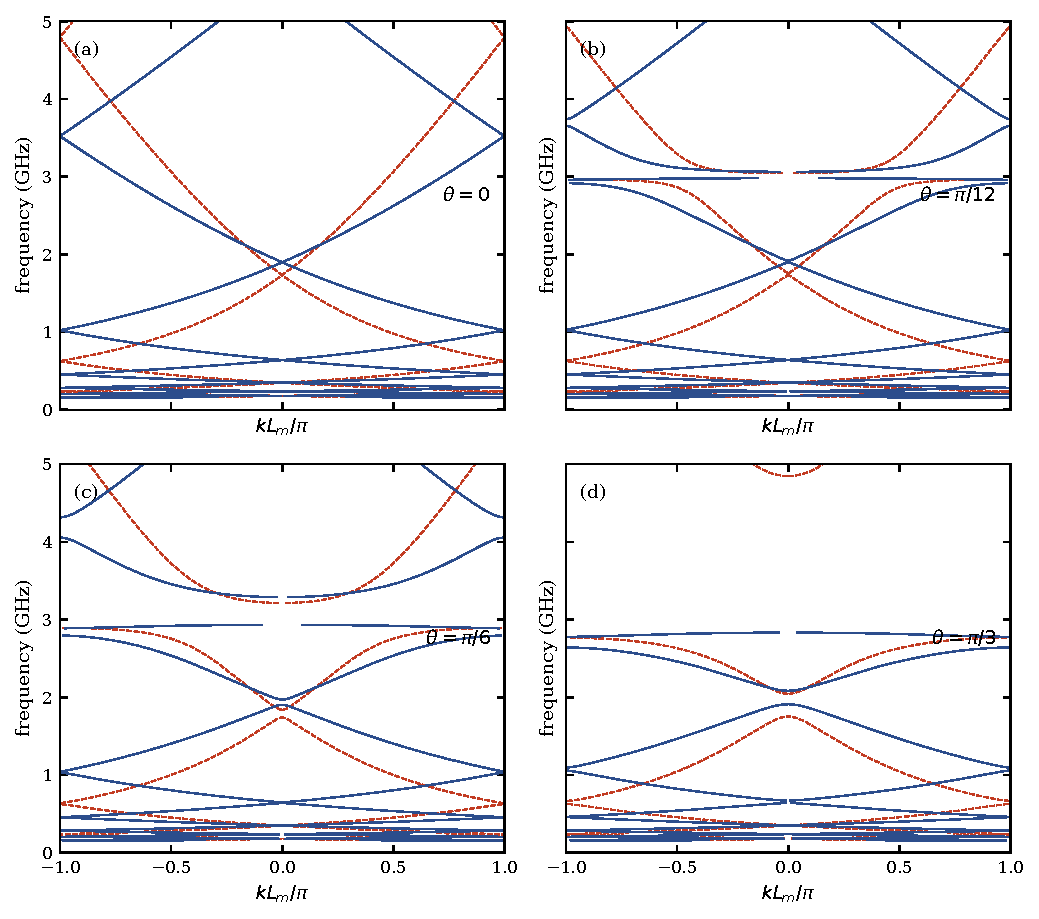
\includegraphics[width=0.92\linewidth]{figure_01/output/figure_01.pdf}
\caption{Reproducción de la Fig.~1: dispersión TE para \(S_3\) y \(S_4\).}
\end{figure}

\subsection{Figura 2}

Zoom cerca de \(\nu_m=3\,\mathrm{GHz}\), \(\theta=\pi/3\), órdenes
\(m=3,4,5,6\).
Debajo de la línea a \(3\,\mathrm{GHz}\) deben verse exactamente
\(1\), \(2\), \(3\) y \(5\) ramas: \(F_{m-2}\).
Es la prueba cuantitativa más limpia del paper.

\begin{figure}[ht]
\centering
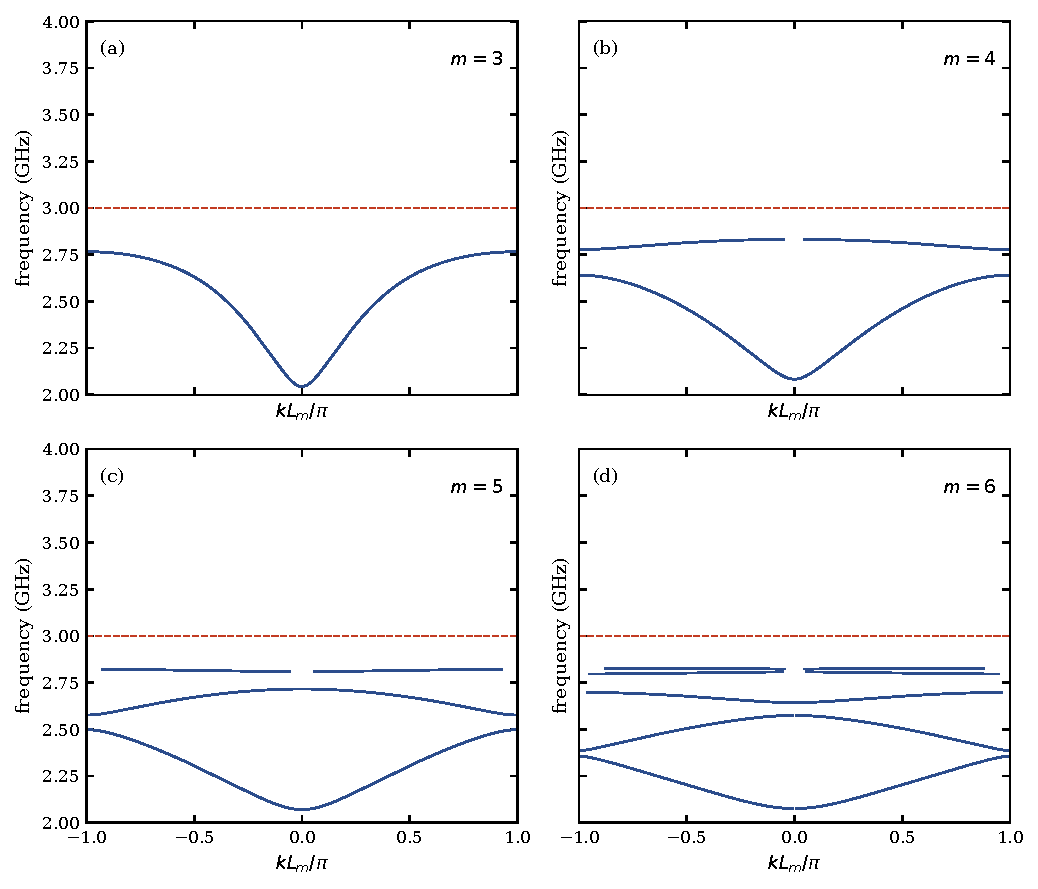
\includegraphics[width=0.92\linewidth]{figure_02/output/figure_02.pdf}
\caption{Reproducción de la Fig.~2. El recuento de ramas es \(F_{m-2}\).}
\end{figure}

\subsection{Figura 3}

Como la Fig.~1, pero \(\nu_m=1\,\mathrm{GHz}\).
A \(\theta=0\) hay un hueco alrededor de \(1\,\mathrm{GHz}\) (el plasmón cae
en el gap \(\langle n\rangle=0\)).
A \(\theta\neq 0\) nace una banda casi horizontal a \(1\,\mathrm{GHz}\): el
polaritón se vuelve ``casi plasmón puro''.
Las bandas altas se desplazan hacia arriba al aumentar \(\theta\).

\begin{figure}[ht]
\centering
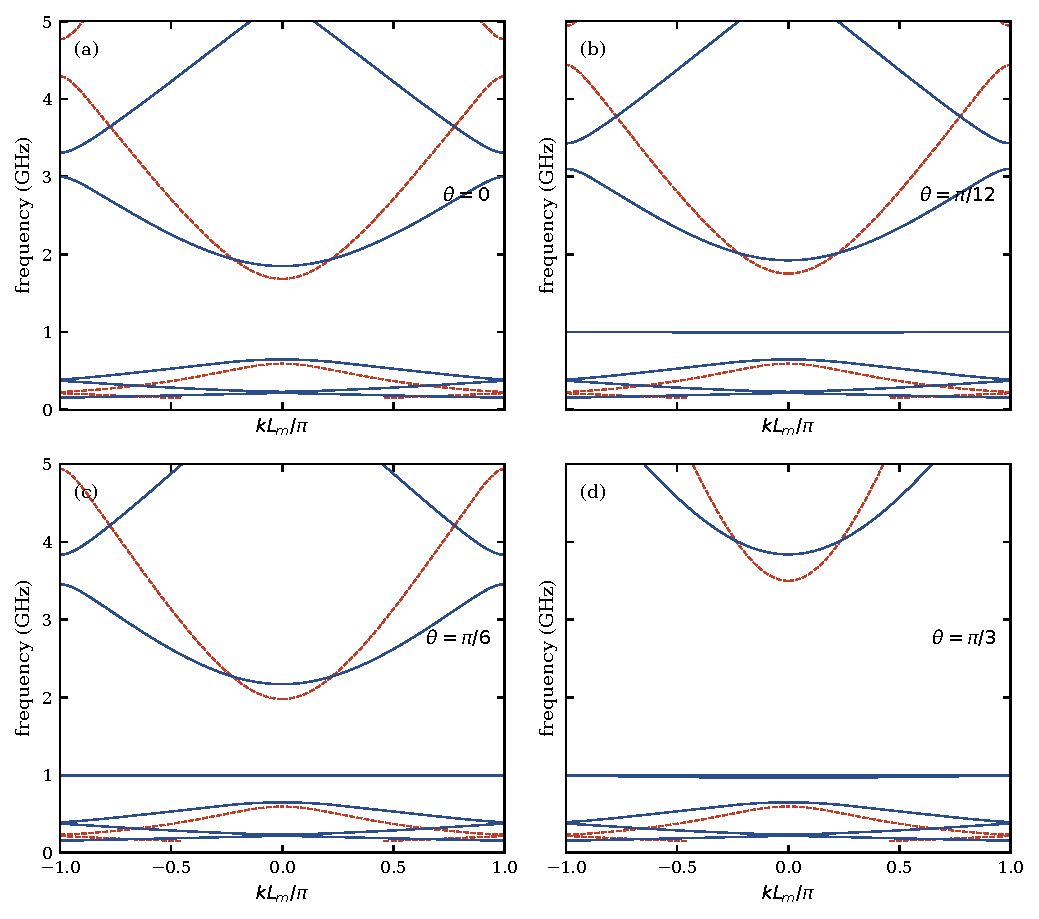
\includegraphics[width=0.92\linewidth]{figure_03/output/figure_03.pdf}
\caption{Reproducción de la Fig.~3. Banda plana en \(1\,\mathrm{GHz}\) solo si
\(\theta\neq 0\).}
\end{figure}

\subsection{Figura 4}

Lupa de esa banda plana, \(m=3\) (una curva) y \(m=4\) (dos).
El ancho \(\Delta\nu=\nu_{\max}-\nu_{\min}\) crece con \(\theta\):
unos \(4.5\,\mathrm{MHz}\) a \(\pi/12\) frente a unos \(33\,\mathrm{MHz}\) a
\(\pi/3\) (el impreso, leído a ojo, sugiere \(\sim 5\) y \(\sim 40\,\mathrm{MHz}\)).
Las curvas son cóncavas hacia arriba, mínimo en \(k=0\).

\begin{figure}[ht]
\centering
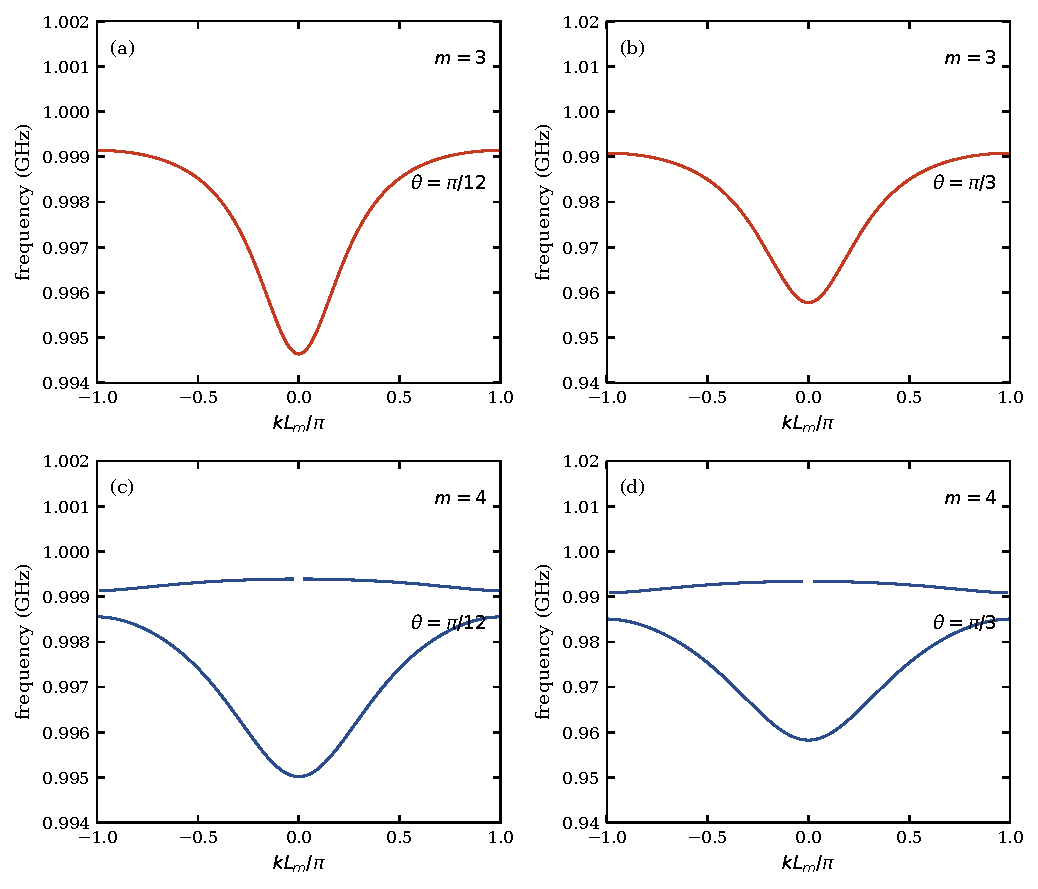
\includegraphics[width=0.92\linewidth]{figure_04/output/figure_04.pdf}
\caption{Reproducción de la Fig.~4. Zoom de los modos plasmon-polaritón.}
\end{figure}

\subsection{Figura 5}

Para cada orden \(m=2,\ldots,8\) se dibuja un segmento vertical por cada
intervalo de frecuencia permitido cerca de \(1\,\mathrm{GHz}\).
\(m=2\) y \(m=3\) tienen un solo segmento (\(F_0=F_1=1\)).
A partir de \(m=4\) hay splitting sucesivo tipo Cantor.
El eje del original está rotulado ``bandwidth (GHz)'', pero los números
(\(0.994\)--\(1.000\) y \(0.95\)--\(1.00\)) son \emph{frecuencias} de las
subbandas; la longitud de cada palo es el ancho.

\begin{figure}[ht]
\centering
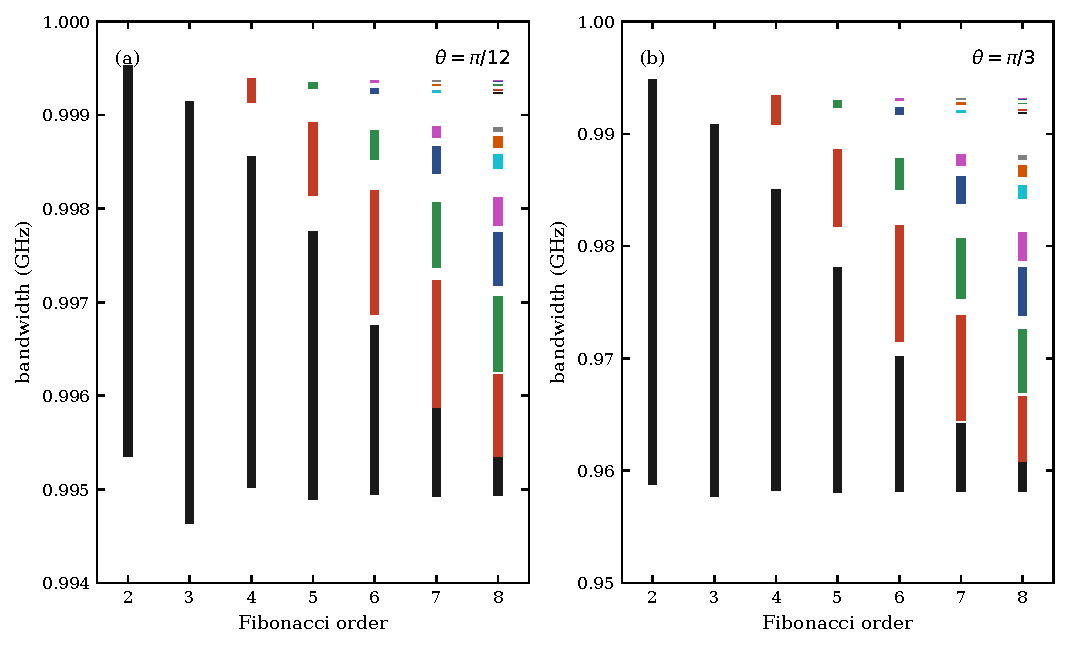
\includegraphics[width=0.92\linewidth]{figure_05/output/figure_05.pdf}
\caption{Reproducción de la Fig.~5. Fragmentación Cantor al subir \(m\).}
\end{figure}

\subsection{Figura 6}

El caption del PRB está truncado. Por contexto se usan los parámetros de las
Figs.\ 3--5 y \(m=2,\ldots,7\).
El original \emph{no} grafica \(\Delta\nu(\theta)\) como una línea que parte de
cero. Grafica la frecuencia de cada subbanda frente a \(\theta\), con la región
entre \(\nu_{\min}\) y \(\nu_{\max}\) rellena.
A \(\theta=0\) las ramas colapsan hacia \(1\,\mathrm{GHz}\); al crecer
\(\theta\) se abren hacia abajo y se parten según \(F_{m-2}\).

\begin{figure}[ht]
\centering
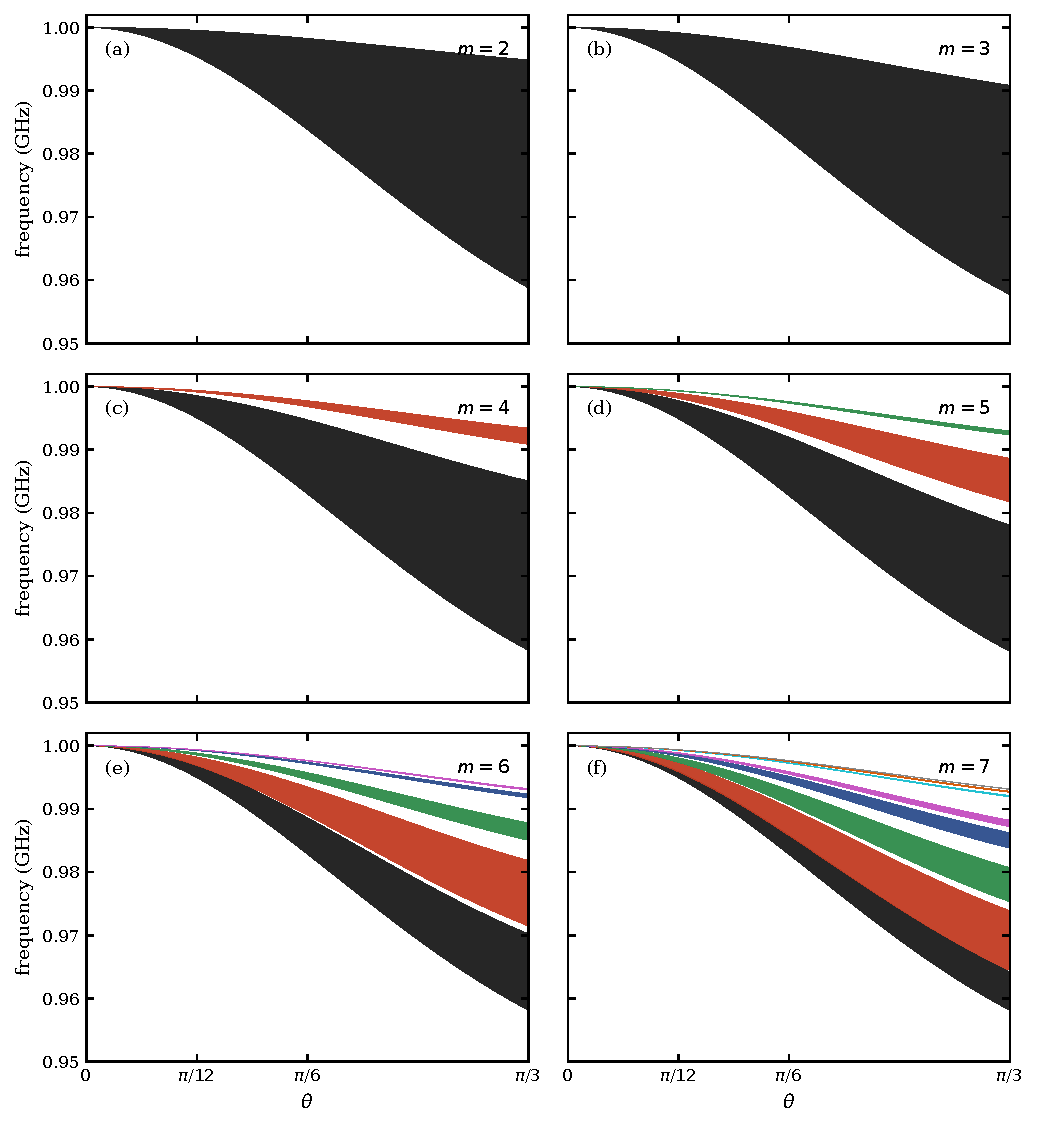
\includegraphics[width=0.78\linewidth]{figure_06/output/figure_06.pdf}
\caption{Reproducción de la Fig.~6 (parámetros inferidos): \(\nu(\theta)\)
relleno.}
\end{figure}

\section{Dos regímenes físicos, una sola fórmula}

Conviene guardar esta dicotomía, porque unifica las seis figuras:

\begin{itemize}
\item \textbf{Figs.\ 1--2.} \(\nu_m\) es una frecuencia \emph{permitida} a
\(\theta=0\). El acoplamiento luz--plasmón es fuerte. Las bandas polaritónicas
son dispersivas (forma de U, anchos de cientos de MHz).
\item \textbf{Figs.\ 3--6.} \(\nu_m\) cae en el gap \(\langle n\rangle=0\).
El acoplamiento se debilita. Las bandas son esencialmente plasmónicas, casi
planas, con anchos de unos pocos a unas decenas de MHz, y espectro tipo Cantor
al subir \(m\).
\end{itemize}

La ecuación \(\cos(k L_m)=R_m\) es la misma. Cambia solo \(\omega_m\).

\section{Qué el paper no especifica}

Ninguno de estos huecos impide replicar las Figs.\ 1--5; todos están
documentados en el código como decisiones de implementación:

\begin{enumerate}
\item El factor \(\omega/c\) en \(q\) (notación de Snell incompleta).
\item El valor numérico de \(c\).
\item La matriz \(2\times 2\) de una capa.
\item La rama de las raíces (\(\varepsilon\), \(\mu\), \(Q\)) en medios LHM.
\item Pérdidas \(\gamma\) (el modelo es sin pérdidas).
\item Resolución del barrido en \(\nu\).
\item Qué hacer cuando \(\lvert R_m\rvert\) vale \(1+10^{-14}\) por redondeo.
\item Caption completo, lista de \(m\) y parámetros de la Fig.\ 6.
\item Perfiles de campo y figuras TM.
\end{enumerate}

No se ajustaron parámetros para ``parecerse'' al dibujo. Donde hay diferencia
visual residual (por ejemplo \(\Delta\nu\) de la Fig.\ 4 versus una lectura a
ojo del impreso) se declara como tal: no hay datos digitales del original.

\section{Glosario}

\begin{description}[style=nextline,leftmargin=1.4cm]
\item[Banda] Intervalo de frecuencia con \(\lvert R_m\rvert\le 1\): la onda
puede propagarse a lo largo de \(z\) con \(k\) real.
\item[Gap (hueco)] \(\lvert R_m\rvert>1\): no hay \(k\) real.
\item[Zona de Brillouin] Intervalo de \(k\) inequívoco de una red periódica;
aquí \(k L_m/\pi\in[-1,1]\).
\item[Celda \(S_m\)] Palabra de Fibonacci que se repite para formar la
superred.
\item[Drude] Modelo \(\varepsilon,\mu=1-\omega_{e,m}^2/\omega^2\).
\item[LHM] Medio con \(\varepsilon<0\) y \(\mu<0\) a la vez.
\item[TMM] Transfer Matrix Method: propagar \(\Psi\) con matrices \(2\times 2\).
\item[Semitraza \(R_m\)] Mitad de la traza de \(T_m\); es \(\cos(k L_m)\).
\item[Polaritón] Modo híbrido fotón + plasmón.
\item[Cantor] Conjunto que se obtiene partiendo un intervalo una y otra vez;
el espectro de Fibonacci tiende a ese patrón al crecer \(m\).
\end{description}

\section{Siguiente lectura}

Con este mapa ya se puede abrir el documento
\textit{Solución numérica e implementación}: allí se recorre, función a
función, cómo el código convierte estas ecuaciones en las seis figuras, qué
barridos usa, cómo decide si un punto es banda o gap, y cómo se dibujan las
curvas sin artefactos.

\begin{thebibliography}{9}
\bibitem{Reyes2010}
E.~Reyes-Gómez, N.~Raigoza, S.~B.~Cavalcanti, C.~A.~A.~de Carvalho y L.~E.~Oliveira,
Phys.\ Rev.\ B \textbf{81}, 153101 (2010).
\bibitem{Reyes2009EPL}
E.~Reyes-Gómez, D.~Mogilevtsev, S.~B.~Cavalcanti, C.~A.~A.~de Carvalho y L.~E.~Oliveira,
EPL \textbf{88}, 24002 (2009).
\bibitem{Kohmoto1983}
M.~Kohmoto, L.~P.~Kadanoff y C.~Tang, Phys.\ Rev.\ Lett.\ \textbf{50}, 1870 (1983).
\bibitem{Veselago1968}
V.~G.~Veselago, Sov.\ Phys.\ Usp.\ \textbf{10}, 509 (1968).
\bibitem{Pendry1996}
J.~B.~Pendry, A.~J.~Holden, W.~J.~Stewart y I.~Youngs, Phys.\ Rev.\ Lett.\ \textbf{76}, 4773 (1996).
\bibitem{Li2003}
J.~Li, L.~Zhou, C.~T.~Chan y P.~Sheng, Phys.\ Rev.\ Lett.\ \textbf{90}, 083901 (2003).
\end{thebibliography}

\end{document}
